\documentclass[11pt,english]{article}
\usepackage[T1]{fontenc}
\usepackage{babel}
\usepackage{graphicx}
\usepackage{hyperref}
\usepackage{rotating}
\usepackage{amsfonts}
\usepackage{amssymb}


\begin{document}
\title{\textit{Deterministic DSA fault attack}}
\author{
  Fabio Gritti\\
  \texttt{fabio1.gritti@mail.polimi.it}
  \and
  Sebastiano Mariani\\
  \texttt{sebastiano.mariani@mail.polimi.it}
  \and \\
  \textbf{Professors}: Gerardo Pelosi , Alessandro Barenghi
}
\date{}
\maketitle

\pagestyle{plain}
\tableofcontents

\section{Introduction}
In this paper we want to introduce two active side channel attacks against the deterministic version of the Digital Signature Algorithm ( from now on DDSA ) as specified in the RFC 6979\cite{rfc}.\\
These attacks can lead directly to a leak of the private key and therefore breaking the authenticity of the signatures created using this algorithm. \\\\
We will proceed in this way: first we provide some useful background in order to understand better the paper, then we explain the attacks in details and finally we present the feasibility of the attack by showing the time needed to break the DSA with some of the keysize currently available.

\section{Background}

\subsection{The Digital Signature Algorithm}

\subsubsection{General overview}
The DSA is one of three digital signature schemes specified in FIPS 186\cite{fips}. A digital signature scheme is an authentication mechanism that enables the creator of a message to attach a code that acts as a signature providing authenticity and non-repudation. \\It usually consists of three algorithms:

\begin{itemize}
\item a \textit{key generation algorithm} that outputs the private key and the corresponding public key.
\item a \textit{signing algorithm} that given a message and a private key produce the signature. 
\item a \textit{signature verifying algorithm} that given a signature and a public key either accepts or rejects the message's claim to authenticity.
\end{itemize}

In order to be a sound digital signature schemes the following properties must hold:

\begin{itemize} 
\item the authenticity of a signature generated from a fixed message and fixed private key can be verified by using the corresponding public key.
\item it should be computationally infeasible to generate a valid signature for a party without knowing that party's private key. 
\item The private key MUST remain private, otherwise the authenticity of the signature created with that key is broken.
\item The public key owner MUST be verifiable, otherwise we can't assure that we had receive a message from a particoular source.
\end{itemize}

\subsubsection{DSA mathematical structure}

The reference group category is ($\mathbb{Z})$) -- COPY FROM SLIDESCOPY FROM SLIDESCOPY FROM SLIDESCOPY FROM SLIDESCOPY FROM SLIDESCOPY FROM SLIDESCOPY FROM SLIDESCOPY FROM SLIDESCOPY FROM SLIDESCOPY FROM SLIDESCOPY FROM SLIDESCOPY FROM SLIDESCOPY FROM SLIDESCOPY FROM SLIDESCOPY FROM SLIDESCOPY FROM SLIDESCOPY FROM SLIDESCOPY FROM SLIDESCOPY FROM SLIDESCOPY FROM SLIDESCOPY FROM SLIDES

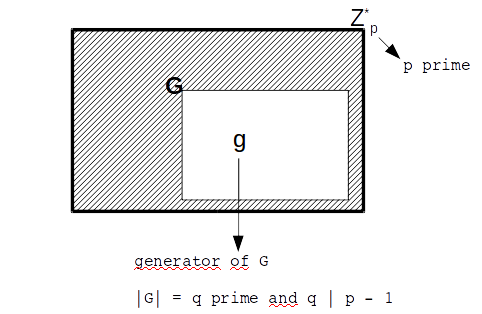
\includegraphics[width=0.8\textwidth]{img_1.png} \\

SLIDESCOPY FROM SLIDESCOPY FROM SLIDESCOPY FROM SLIDESCOPY FROM SLIDESCOPY FROM SLIDESCOPY FROM SLIDESCOPY FROM SLIDESCOPY FROM SLIDESCOPY FROM SLIDESCOPY FROM SLIDESCOPY FROM SLIDESCOPY FROM SLIDESCOPY FROM SLIDESCOPY FROM SLIDESCOPY FROM SLIDESCOPY FROM SLIDES

\subsubsection{Cryptoscheme}

SLIDESCOPY FROM SLIDESCOPY FROM SLIDESCOPY FROM SLIDESCOPY FROM SLIDESCOPY FROM SLIDESCOPY FROM SLIDESCOPY FROM SLIDESCOPY FROM SLIDESCOPY FROM SLIDESCOPY FROM SLIDESCOPY FROM SLIDESCOPY FROM SLIDESCOPY FROM SLIDESCOPY FROM SLIDESCOPY FROM SLIDESCOPY FROM SLIDES

\subsection{The Deterministic Digital Signature Algorithm}

\subsubsection{General overview}
The step in the signing algorithm that require to generate a random parameter needs a great randomness in order to be secure; but digging with embedded system not always we have on board a sound RNG! \\This is the crucial point for which many manufacturers decide to employ RSA cryptosystem rather than DSA/ECDSA to sign objects.\\
\\The Deterministic DSA proposed in the RFC 6979 try to make that step deterministic in order to increase the attractiveness of such system in the embedded world ( smart card, credit card etc... ).\\\\
Remember that we ,in any way, need a good RNG in order to generate a strong private key. 
This proposal make deterministic the signing, NOT the generation of keys that MUST be non deterministic and made a priopri.


\subsubsection{K deterministic generation}

The generation of the deterministic \textit{k} depends only from the message to sign and the private key.\\
According to the RFC ,  given the input message m, the following process is applied for the generation:

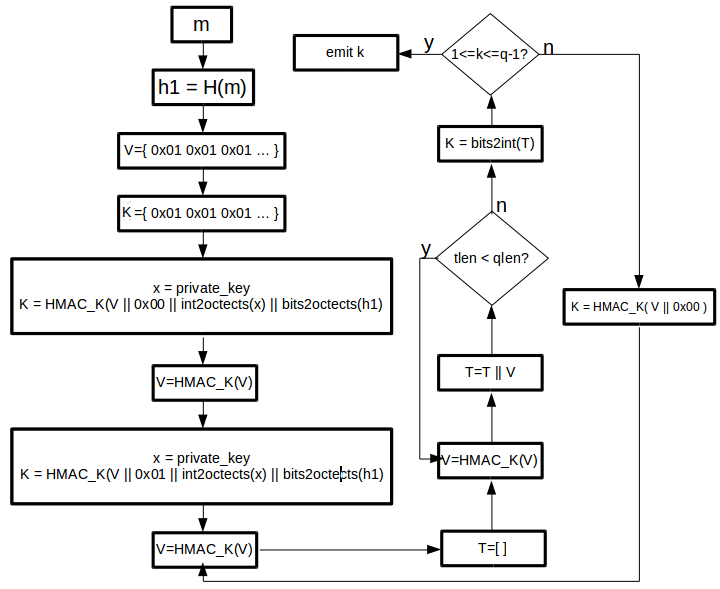
\includegraphics[width=1.0\textwidth]{img_2.png} \\

\begin{itemize}
\item qlen = binary length of the prime number \textit{q}
\item tlen = binary length of the array T 
\item The internal HMAC use the same hash function used in the h1=H(m)
\end{itemize}

\subsection{Other asymmetric deterministic algorithm}

dECDSA  + EdDSA -- Bernstein

\section{Cracking the Deterministic DSA}

\subsection{Differential fault analysis}

The differential fault analysis is an active side channel attack that is performed in three steps:
\begin{itemize}
\item Obtain the correct signature of a message.
\item Inject a fault during a second signing of the message and obtain the \textit{faulty signature}.
\item Correlate the correct signature with the faulty one and extract the private key.
\end{itemize}

In order to inject a fault we can use different techniques that range from using laser beam during the signing process, to voltage spike, insane overclocking etc..
\\Usually critical embedded systems like credit card implements different defenses against this fault injection techniques; this raise a lot the cost of an attack performed by an attacker. \\Bypass this kind of defense is out of scope of this paper.

\subsection{The attack in practice}

INFO SULLE LIBRERIE USATE ( libgcrypt ) 

\subsubsection{Breaking the exponentation}

\subsubsection{Breaking the signature composition}

\section{Results}

\subsection{Breaking the exponentation}

FARE TEST CON STESSO FAULT SUL BIT

\subsection{Breaking the signature composition}

FARE TIMING TEST CON STESSO FAULT SUL BIT
FARE TIMING TEST CON STESSO FAULT SUL BYTE 

\section{Conclusion}

\addcontentsline{toc}{section}{\refname}
\begin{thebibliography}{10}
\bibitem{rfc} https://tools.ietf.org/html/rfc6979
\bibitem{fips} http://nvlpubs.nist.gov/nistpubs/FIPS/NIST.FIPS.186-4.pdf

\end{thebibliography}

\end{document}
